% EXEC_14 — Beamer compendium EJ-204 vs EJ-230
% SHiP Timing Detector Collaboration Meeting, 15–16 June 2026
% QA-3b: translated to EN; ToF diagram slide; 3 content fixes; F7 order-statistics
% Compile: lualatex exec14_deck.tex && lualatex exec14_deck.tex
\documentclass[aspectratio=169,9pt]{beamer}

% ── Theme ─────────────────────────────────────────────────────────────────────
\usetheme{Madrid}
\usecolortheme{default}
\setbeamertemplate{navigation symbols}{}
\setbeamerfont{frametitle}{size=\normalsize,series=\bfseries}
\setbeamerfont{framesubtitle}{size=\small}

% ── Fonts (LuaLaTeX) ─────────────────────────────────────────────────────────
\usepackage{fontspec}
\setsansfont{DejaVu Sans}[Scale=0.93]
\setmonofont{DejaVu Sans Mono}[Scale=0.85]

% ── Packages ──────────────────────────────────────────────────────────────────
\usepackage{graphicx}
\usepackage{booktabs}
\usepackage{xcolor}
\usepackage{siunitx}
\sisetup{separate-uncertainty=true}
\usepackage{tikz}
\usetikzlibrary{arrows.meta}

\graphicspath{{outputs/}}

% ── Colors ────────────────────────────────────────────────────────────────────
\definecolor{ej204col}{HTML}{1f78b4}
\definecolor{ej230col}{HTML}{e31a1c}
\definecolor{okgreen}{HTML}{2ca02c}
\definecolor{pendgold}{HTML}{d4a017}

% ── Metadata ──────────────────────────────────────────────────────────────────
\title[EJ-204 vs EJ-230 — SHiP Timing]{%
  Optical Simulation of Scintillator Bars\\
  \large EJ-204 vs EJ-230 for the SHiP Timing Detector}
\author[R.~Ríos / G.~Vásquez]{%
  René Ríos \and Gerardo Vásquez}
\institute[SHiP Timing]{SHiP Collaboration — Timing Detector Group}
\date{15--16 June 2026}

% ══════════════════════════════════════════════════════════════════════════════
\begin{document}

\begin{frame}[plain]
  \titlepage
\end{frame}

\begin{frame}{Contents}
  \tableofcontents
\end{frame}

% ══════════════════════════════════════════════════════════════════════════════
\section{Setup and geometry}

\begin{frame}{Bar geometry and SiPM readout}
  \begin{columns}[T]
    \begin{column}{0.50\textwidth}
      \textbf{Scintillator bar (GEANT4):}
      \begin{itemize}
        \item Active length: \SI{1400}{\mm} ($\pm700$\,mm along $x$)
        \item Coating: reflective Mylar
        \item $v_\text{eff}\approx277$\,mm/ns (nominal axial average)
        \item[$\hookrightarrow$] {\footnotesize ToF onset measures $v_\text{eff}^\text{onset}\approx292$\,mm/ns
              ($+5\%$): set by the most direct rays, not the mean path (see QA-1c)}
        \item Two materials compared in parallel:\\
              \textcolor{ej204col}{\textbf{EJ-204}} vs
              \textcolor{ej230col}{\textbf{EJ-230}}
      \end{itemize}
      \vspace{0.2em}
      \textbf{End SiPMs (primary timing):}
      \begin{itemize}
        \item 16 SiPMs total (IDs 0–15)
        \item END\_LEFT: IDs 0–7 at $x=-700$\,mm
        \item END\_RIGHT: IDs 8–15 at $x=+700$\,mm
        \item Timing estimator: \textbf{SUM4} ($\min$ over 4-neighbor clusters)
      \end{itemize}
    \end{column}
    \begin{column}{0.48\textwidth}
      \textbf{Top SiPMs (veto / tracking):}
      \begin{itemize}
        \item 70 SiPMs, single row at $Y=+30.25$\,mm
        \item TOP\_LEFT: IDs 16–50 / TOP\_RIGHT: 51–85
        \item Pitch: \SI{20}{\mm} in $X$; central gap \SI{24}{\mm}
      \end{itemize}
      \vspace{0.3em}
      \textbf{GEANT4 statistics:}
      \begin{center}
        \small
        \begin{tabular}{lrr}
          \toprule
          Dataset & Events & Positions \\
          \midrule
          EJ-204 End & 2000/pos & 31 \\
          EJ-230 End & 2000/pos & 31 \\
          EJ-204 EndTop & 2000/pos & 31 \\
          \bottomrule
        \end{tabular}\\[0.2em]
        {\footnotesize Positions: $x = 0, \pm50, \ldots, \pm690$\,mm}
      \end{center}
    \end{column}
  \end{columns}
\end{frame}

% ══════════════════════════════════════════════════════════════════════════════
\section{Photon arrival-time profile — F1}

\begin{frame}{F1: Relative arrival time $t_\text{rel}$ — central position $x=0$}
  \framesubtitle{%
    \textcolor{ej204col}{\textbf{EJ-204}} (left) vs
    \textcolor{ej230col}{\textbf{EJ-230}} (right) —
    1-mode fit: $N(1-e^{-t/\tau_r})\,e^{-t/\tau_f}$}
  \begin{columns}[c]
    \begin{column}{0.49\textwidth}
      \centering
      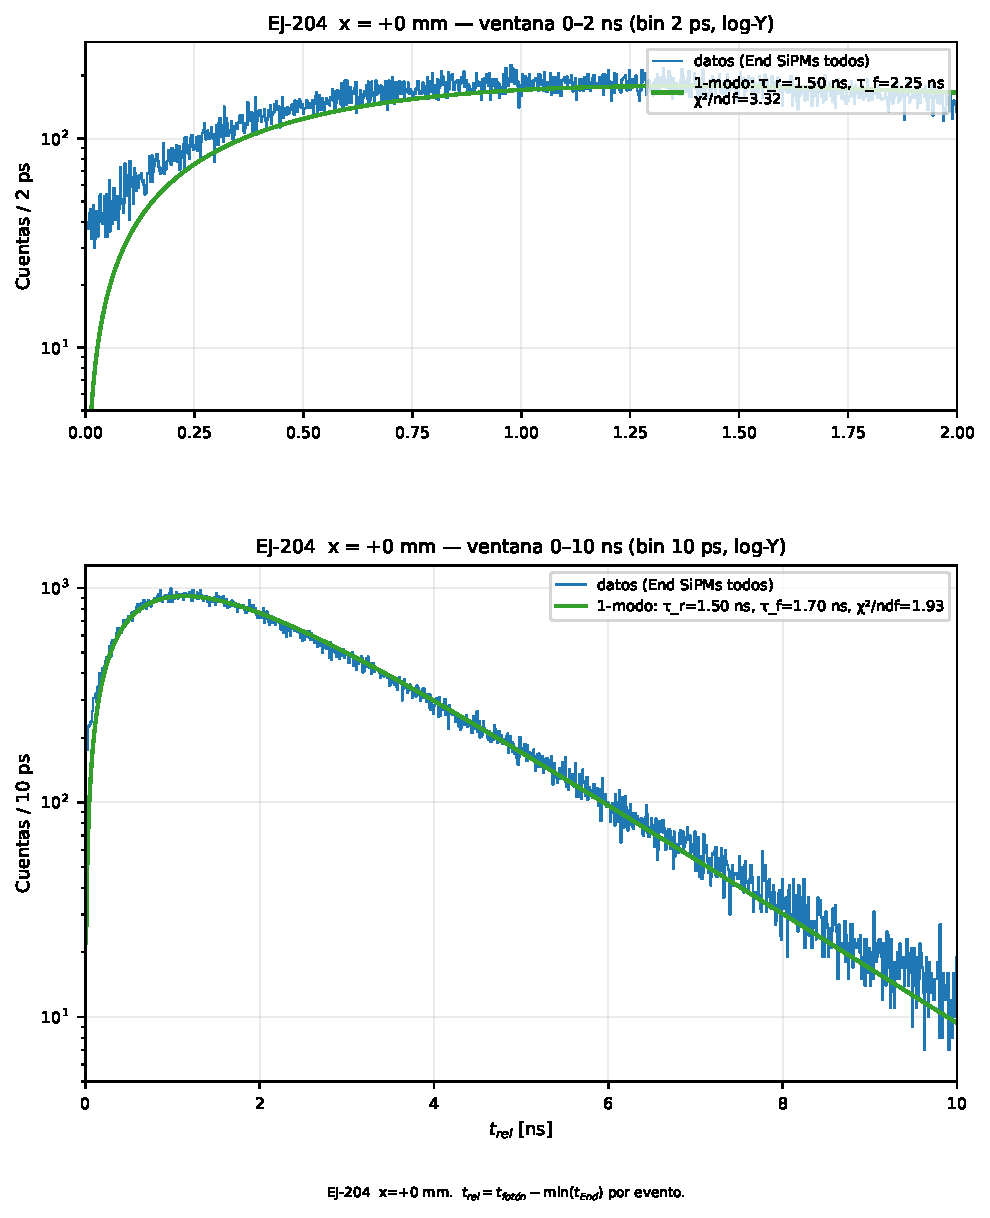
\includegraphics[height=0.60\textheight,keepaspectratio]{fig01a.pdf}
    \end{column}
    \begin{column}{0.49\textwidth}
      \centering
      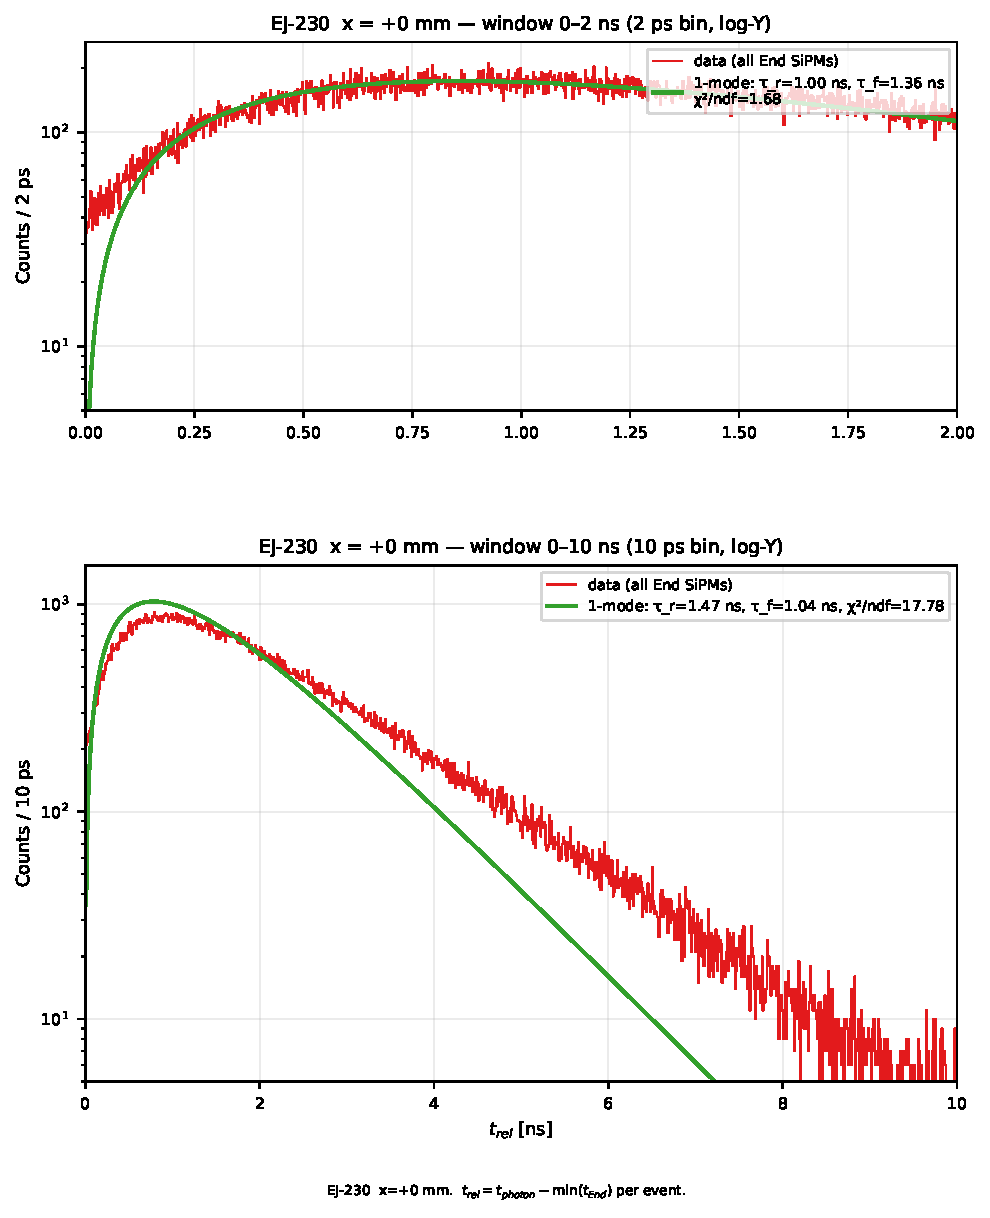
\includegraphics[height=0.60\textheight,keepaspectratio]{fig01d.pdf}
    \end{column}
  \end{columns}
  \vspace{0.1em}
  \begin{center}
    {\footnotesize
      $t_\text{rel}=t_\text{photon}-\min(t_\text{End})$ per event. \quad
      EJ-204: $\tau_r=1.50$\,ns, $\tau_f=1.70$\,ns ($\chi^2/\text{ndf}=1.93$). \quad
      EJ-230: $\tau_r=1.47$\,ns, $\tau_f=1.04$\,ns ($\chi^2/\text{ndf}=17.8$). \\[0.2em]
      \textit{Fitted $\tau$ describe the arrival-time profile (emission $\otimes$ propagation),
      NOT the datasheet emission constants (EJ-204: $\tau_r^{(0)}=0.7$\,ns, $\tau_d^{(0)}=1.8$\,ns).} \\
      EJ-230 tail at $x=0$: \textbf{cannot} be ToF (ends equidistant);
      origin undetermined — slow mode vs reflections.}
  \end{center}
\end{frame}

\begin{frame}{F1: Relative arrival time $t_\text{rel}$ — edge position $x=+690$\,mm}
  \framesubtitle{Second component at $\sim4.7$\,ns visible in both materials}
  \begin{columns}[c]
    \begin{column}{0.49\textwidth}
      \centering
      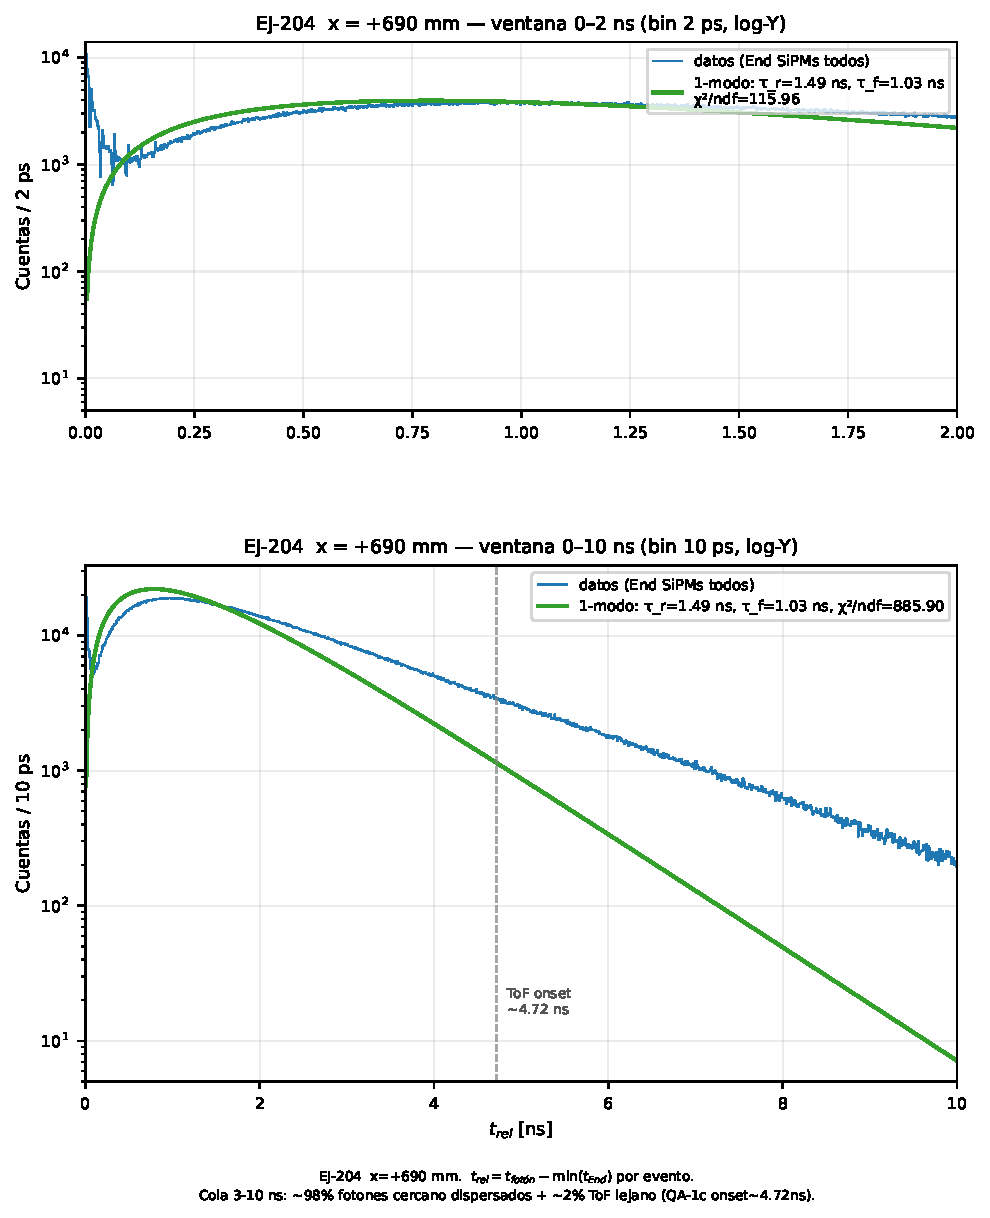
\includegraphics[height=0.70\textheight,keepaspectratio]{fig01c.pdf}
    \end{column}
    \begin{column}{0.49\textwidth}
      \centering
      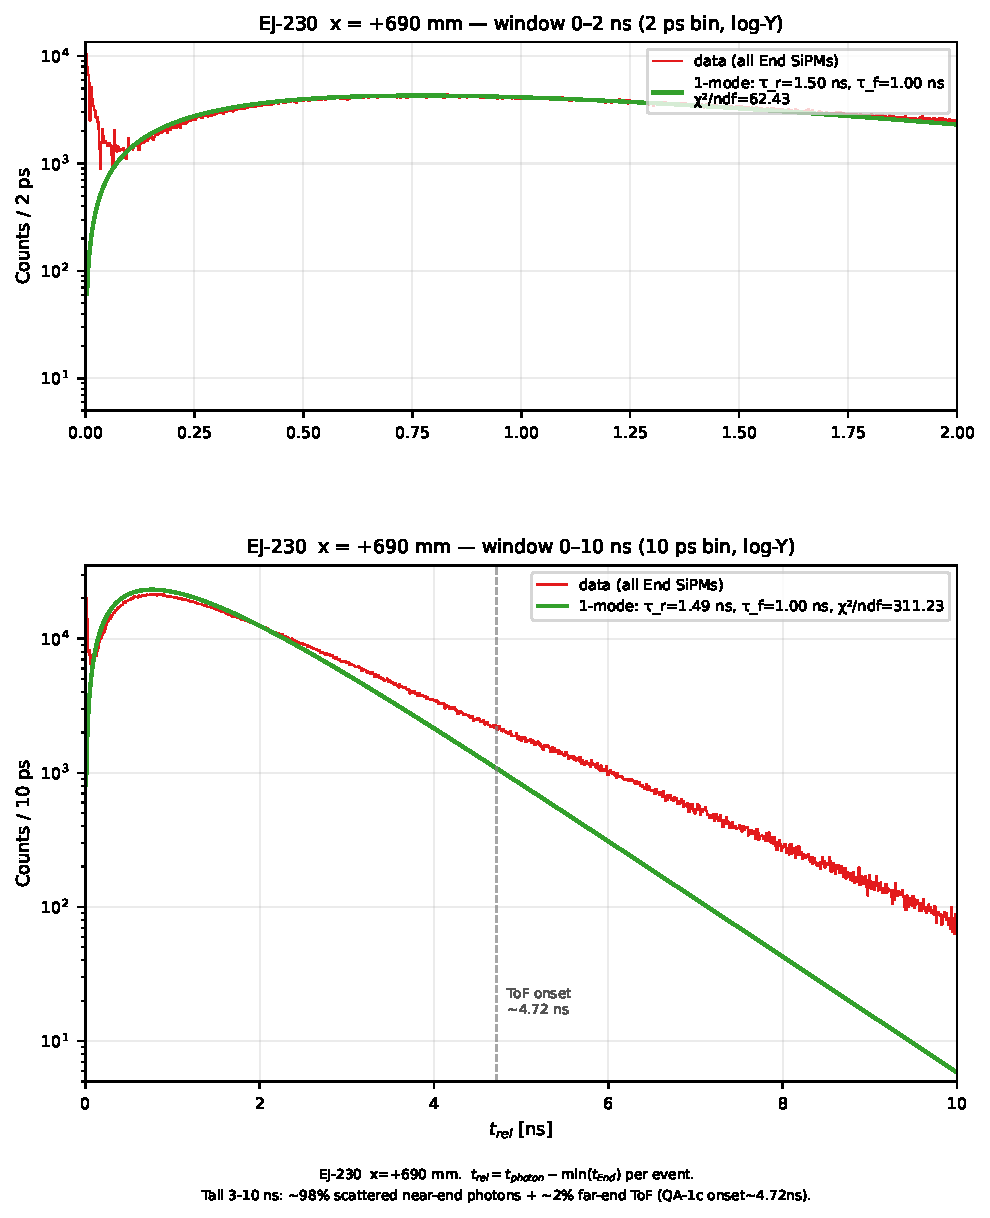
\includegraphics[height=0.70\textheight,keepaspectratio]{fig01f.pdf}
    \end{column}
  \end{columns}
  \vspace{0.2em}
  \begin{center}
    {\footnotesize
      1-mode fit fails at $x=+690$: $\chi^2/\text{ndf}=886$ (EJ-204), $721$ (EJ-230). \quad
      Tail 3--8\,ns: \textbf{not} slow scintillation — see ToF diagram below and QA-1c.}
  \end{center}
\end{frame}

% ══════════════════════════════════════════════════════════════════════════════
\section{Geometric time-of-flight — QA-1c}

% ── NEW SLIDE: ToF diagram ───────────────────────────────────────────────────
\begin{frame}{Why a second component appears at the edge — geometric time-of-flight}
  \begin{center}
  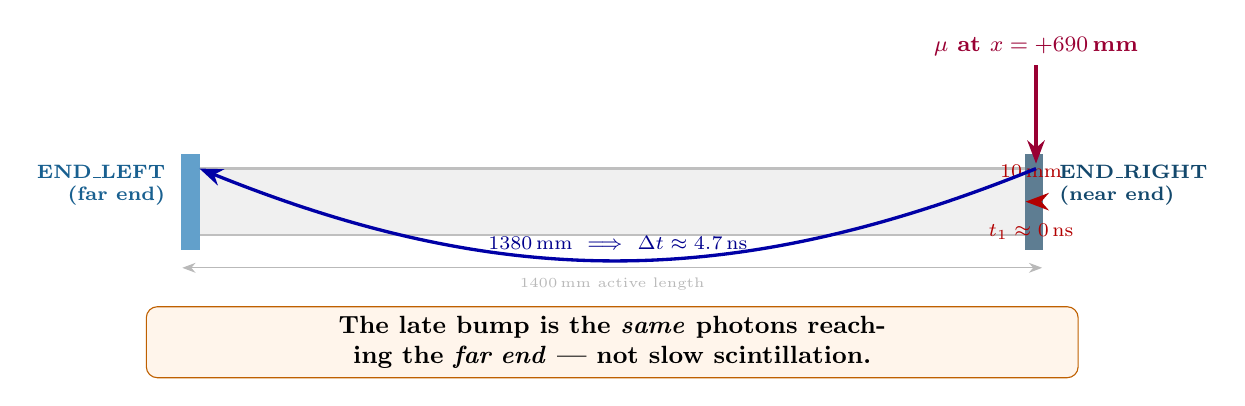
\begin{tikzpicture}[x=0.78cm, y=1.05cm, >=Stealth]

    % ── Bar body ──────────────────────────────────────────────────────────────
    \fill[gray!12] (-7,-0.40) rectangle (7,0.40);
    \draw[thick, gray!50] (-7,-0.40) rectangle (7,0.40);

    % ── END_LEFT SiPM (far end at x=-700 mm) ─────────────────────────────────
    \fill[ej204col!70] (-7.02,-0.58) rectangle (-6.72,0.58);
    \node[left, font=\scriptsize\bfseries, text=ej204col!80!black, align=right]
        at (-7.12, 0.20) {END\_LEFT\\(far end)};

    % ── END_RIGHT SiPM (near end at x=+700 mm) ───────────────────────────────
    \fill[ej204col!35!gray] (6.72,-0.58) rectangle (7.02,0.58);
    \node[right, font=\scriptsize\bfseries, text=ej204col!60!black, align=left]
        at (7.12, 0.20) {END\_RIGHT\\(near end)};

    % ── Muon at x=+690 mm (≈ +6.9 units) ────────────────────────────────────
    \draw[very thick, purple!80!black, ->] (6.90,1.65) -- (6.90,0.46);
    \node[above, font=\footnotesize\bfseries, text=purple!80!black]
        at (6.90,1.65) {$\mu$\ at\ $x=+690$\,mm};

    % ── Short path to near end (10 mm, ~0 ns) ────────────────────────────────
    \draw[very thick, red!70!black, ->] (6.90, 0.0) -- (6.73, 0.0);
    \node[above, font=\scriptsize, text=red!70!black] at (6.82, 0.18) {10\,mm};
    \node[below, font=\scriptsize, text=red!70!black] at (6.82,-0.15) {$t_1\approx0$\,ns};

    % ── Long path to far end (1380 mm, ~4.7 ns) — curved arc above bar ───────
    \draw[very thick, blue!65!black, ->]
        (6.90, 0.40) to[bend left=22]
        node[above, pos=0.50, font=\scriptsize, text=blue!55!black]
        {1380\,mm \ $\Longrightarrow$ \ $\Delta t \approx 4.7$\,ns}
        (-6.72, 0.40);

    % ── Bar length annotation ─────────────────────────────────────────────────
    \draw[<->, gray!55, thin] (-7,-0.80) -- (7,-0.80);
    \node[below, gray!55, font=\tiny] at (0,-0.80) {1400\,mm active length};

    % ── Key message ──────────────────────────────────────────────────────────
    \node[draw=orange!75!black, fill=orange!8, rounded corners=4pt,
          text width=11.6cm, align=center, font=\small\bfseries]
        at (0,-1.70)
        {The late bump is the \emph{same} photons reaching the \emph{far end} —
         not slow scintillation.};

  \end{tikzpicture}
  \end{center}
\end{frame}

\begin{frame}{QA-1c: Second F1 component confirmed as geometric ToF}
  \begin{columns}[c]
    \begin{column}{0.63\textwidth}
      \centering
      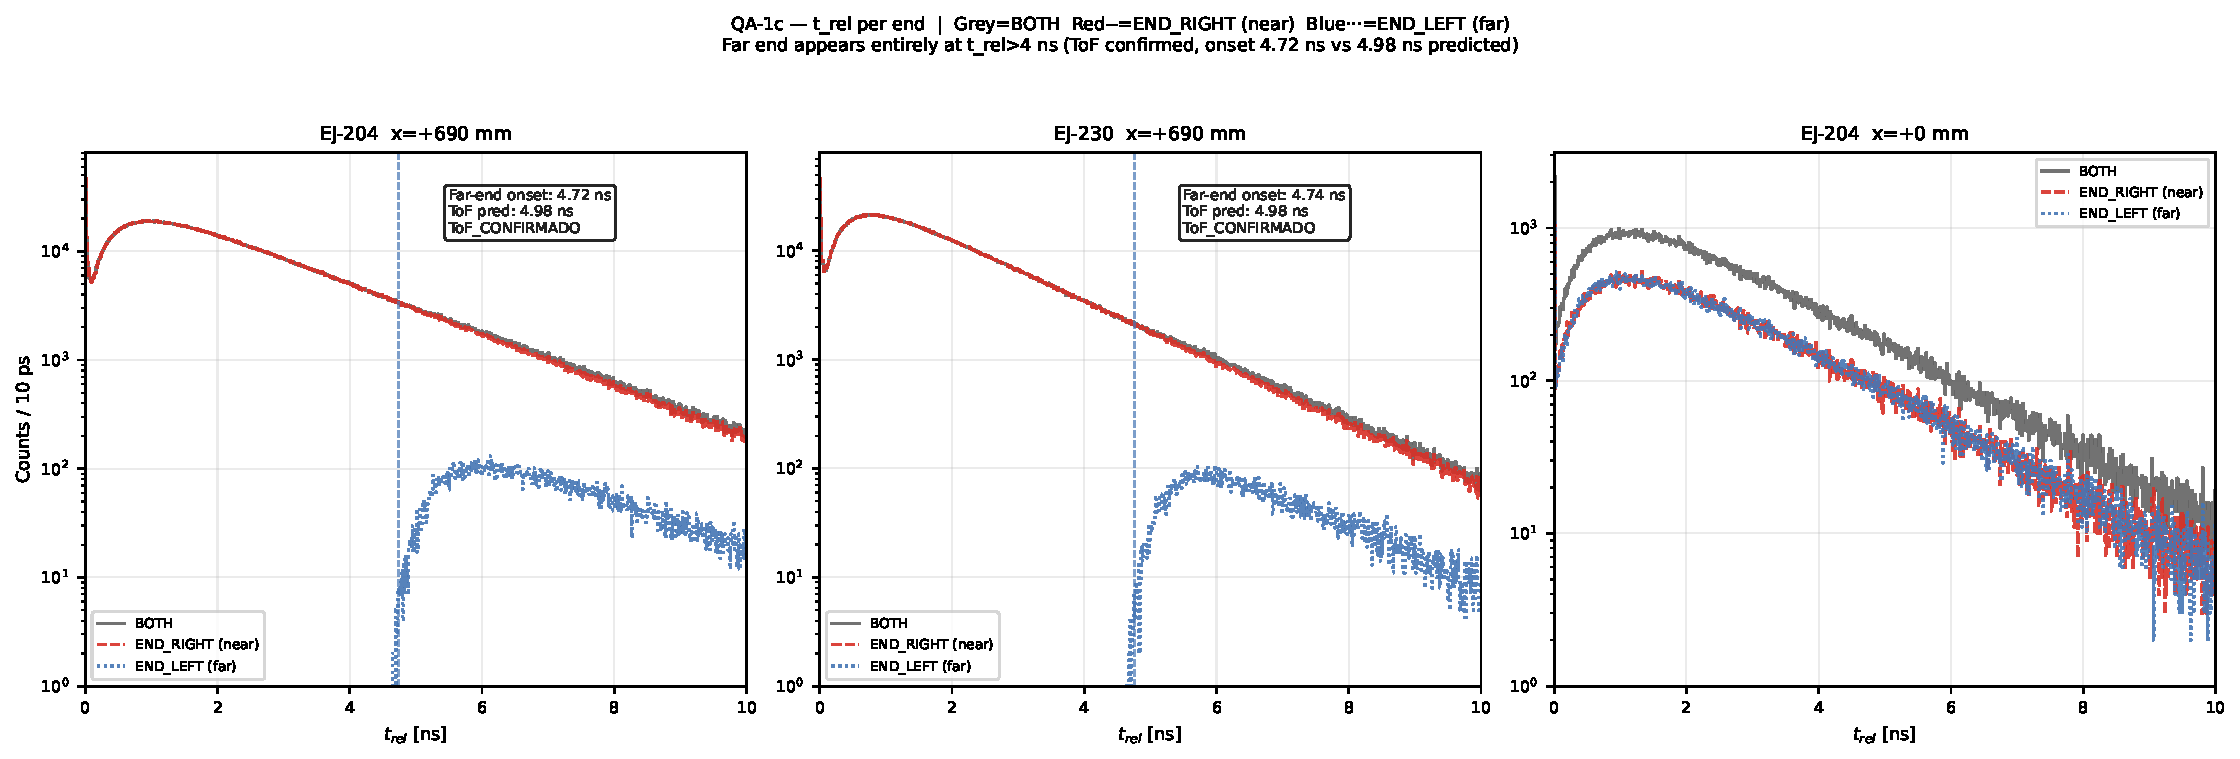
\includegraphics[width=\textwidth,keepaspectratio]{fig01_tof_probe_vis.pdf}
    \end{column}
    \begin{column}{0.35\textwidth}
      \textbf{ToF prediction ($x=+690$\,mm):}
      \[
        \Delta t_\text{pred} = \frac{1380\,\text{mm}}{277\,\text{mm/ns}}
        \approx 4.98\,\text{ns}
      \]

      \textbf{Measured onset (far end):}
      \begin{itemize}
        \item \textcolor{ej204col}{EJ-204}: $4.72$\,ns \hfill $(-5.3\%)$
        \item \textcolor{ej230col}{EJ-230}: $4.74$\,ns \hfill $(-4.9\%)$
      \end{itemize}

      \vspace{0.4em}
      \textbf{Verdict:}\\
      \textcolor{okgreen}{\textbf{ToF\_CONFIRMED}}\\[0.3em]
      {\footnotesize
        The $-5\%$ offset reflects $v_\text{eff}^\text{onset}\approx292$\,mm/ns
        — the fastest (most direct) optical rays arrive first,
        pulling the onset earlier than the mean-path prediction.}
    \end{column}
  \end{columns}
\end{frame}

% ══════════════════════════════════════════════════════════════════════════════
\section{Spatial hit distribution — F3}

\begin{frame}{F3: Spatial distribution of photon impacts on SiPMs}
  \framesubtitle{Single representative event — EJ-204 (EJ-230 qualitatively identical)}
  \begin{columns}[c]
    \begin{column}{0.49\textwidth}
      \centering
      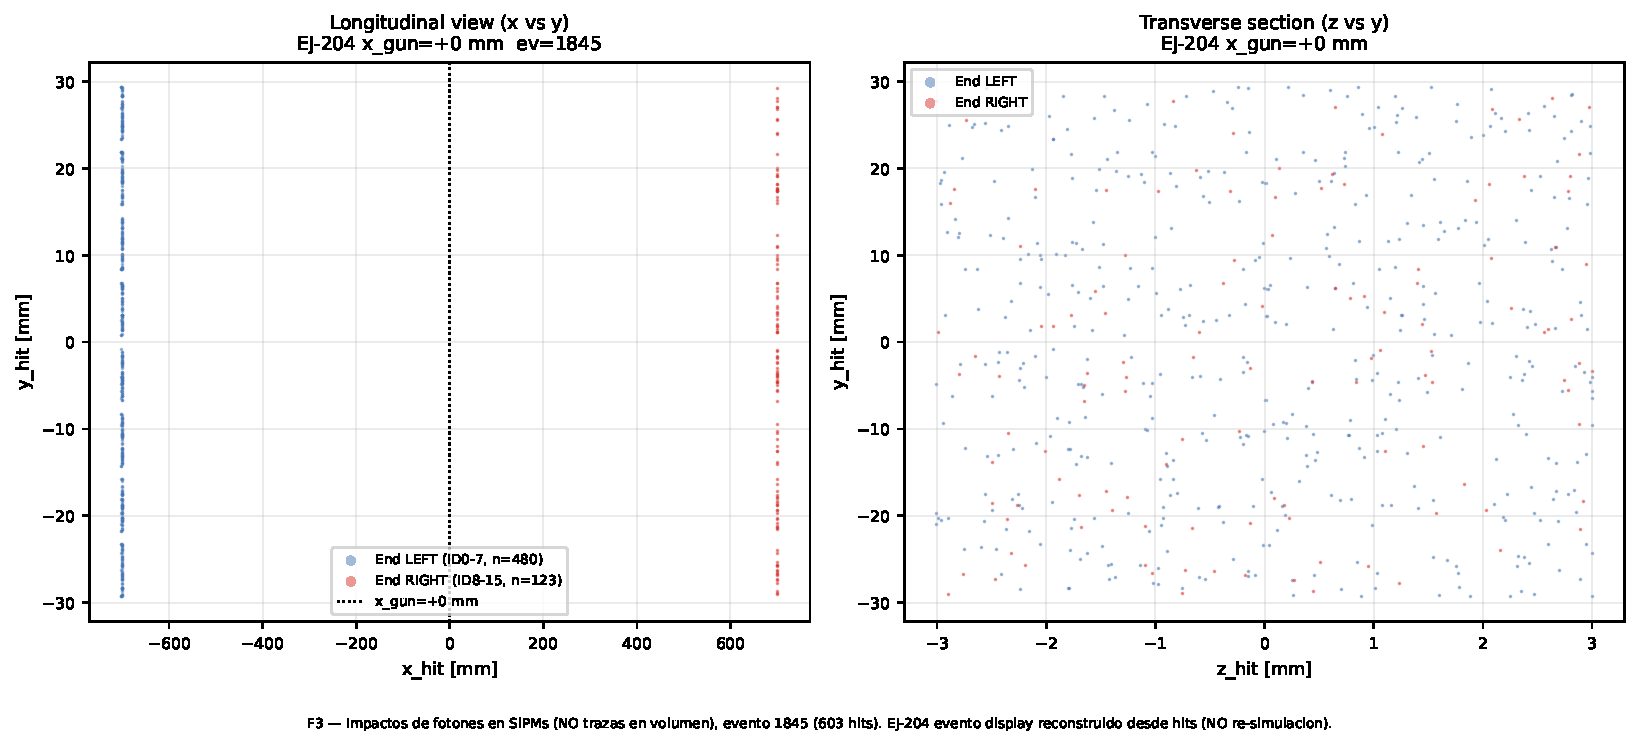
\includegraphics[width=\textwidth,keepaspectratio]{fig03a.pdf}\\
      {\footnotesize $x_\text{gun}=0$\,mm — symmetric L/R distribution}
    \end{column}
    \begin{column}{0.49\textwidth}
      \centering
      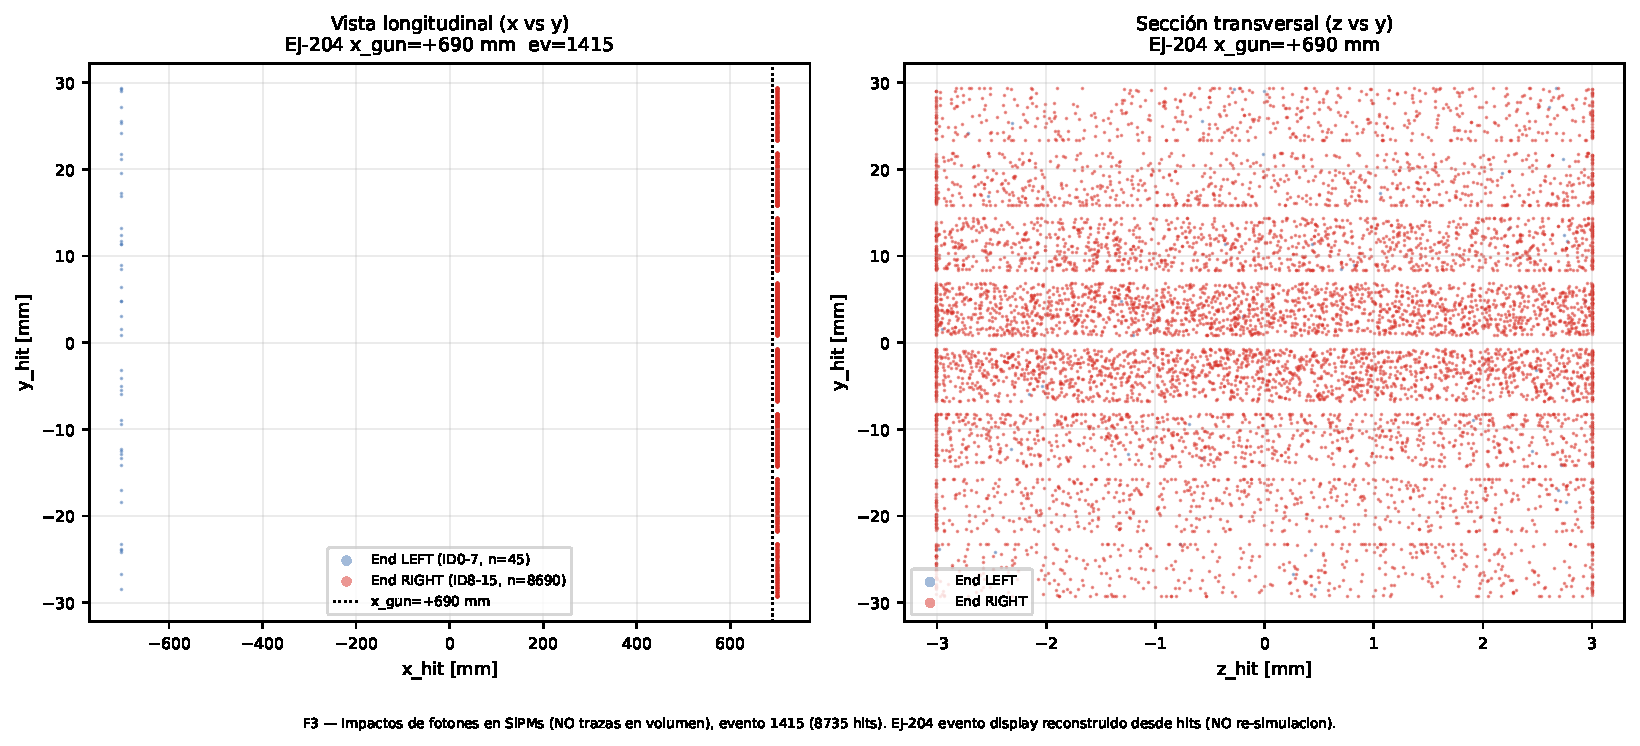
\includegraphics[width=\textwidth,keepaspectratio]{fig03b.pdf}\\
      {\footnotesize $x_\text{gun}=+690$\,mm — collapse toward END\_RIGHT}
    \end{column}
  \end{columns}
  \vspace{0.2em}
  {\footnotesize
    \textit{Note:} Points are \emph{photon impacts on the SiPM window}
    (NOT trajectories inside the scintillator volume). Proxy of optical propagation.
    Reconstructed from \texttt{x\_mm}/\texttt{y\_mm}/\texttt{z\_mm} ROOT branches — no re-simulation.}
\end{frame}

% ══════════════════════════════════════════════════════════════════════════════
\section{$\sigma_t$ vs $N_{pe}$ and Top profiles — F2, F4}

\begin{frame}{F2: $\sigma_t$ vs $N_{pe}$ (END SiPMs) — pure Poisson, more light always helps}
  \begin{columns}[c]
    \begin{column}{0.48\textwidth}
      \centering
      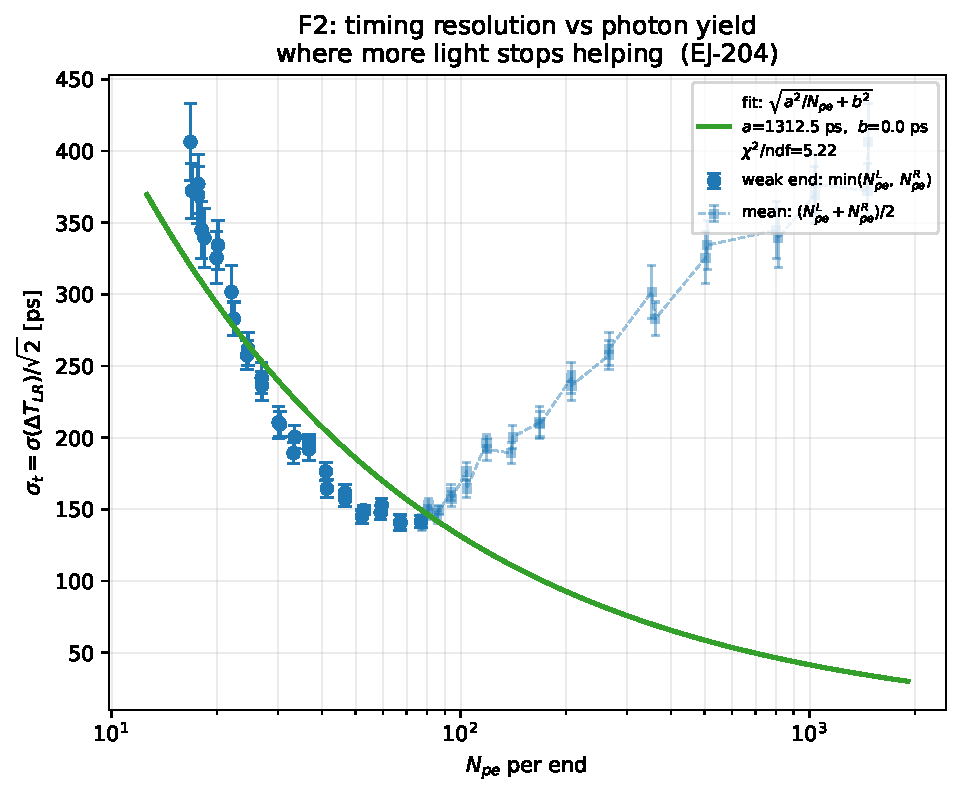
\includegraphics[width=\textwidth,keepaspectratio]{fig02a.pdf}
    \end{column}
    \begin{column}{0.48\textwidth}
      \centering
      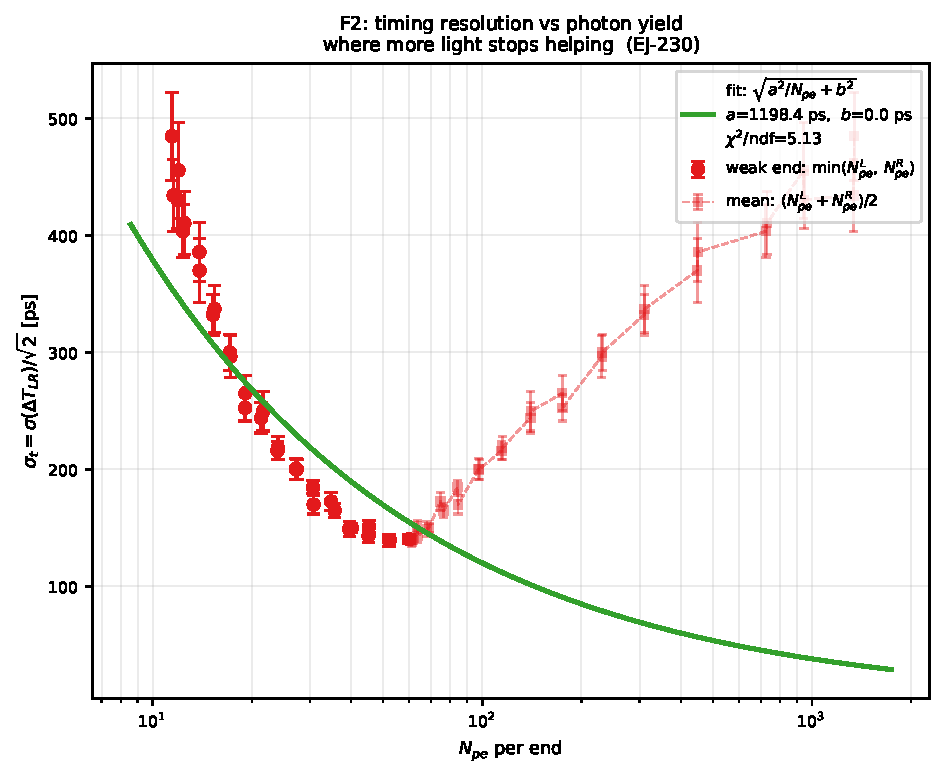
\includegraphics[width=\textwidth,keepaspectratio]{fig02b.pdf}
    \end{column}
  \end{columns}
  \vspace{0.05em}
  {\tiny
  \textbf{END SiPMs} (IDs 0–15, timing); each point = one muon position;
  $x\!=\!N_{pe}^\text{weak}$ (far-end photons); $y\!=\!\sigma_t$ (same as F5).
  \emph{For Top SiPM light profiles, see F4.}\\[0.1em]
  \textcolor{ej204col}{\textbf{EJ-204}}: $a=1312\pm24$\,ps,\;$b=0$,\;$\chi^2/\text{ndf}=5.22$
  \quad
  \textcolor{ej230col}{\textbf{EJ-230}}: $a=1198\pm23$\,ps,\;$b=0$,\;$\chi^2/\text{ndf}=5.13$\\[0.1em]
  \textbf{Pure Poisson} ($\sigma_t\!\propto\!1/\!\sqrt{N_{pe}}$, $b=0$):
  no saturation in $N_{pe}^\text{weak}\!\in[11,77]$.
  \textbf{Edge timing is limited by \emph{scarce far-end light}, not by propagation spread.
  Adding light always improves edge timing.}\\[0.1em]
  \textit{F2\,\&\,F7 consistent}: optical-path dispersion EXISTS (F7 RMS\,>\,floor) but
  \emph{subdominant} to Poisson statistics in SUM4 $\sigma_t$ ($b\!\approx\!0$).}
\end{frame}

\begin{frame}{F4: Top SiPM light yield vs position — \textbf{not} a timing quantity (EndTop EJ-204)}
  \centering
  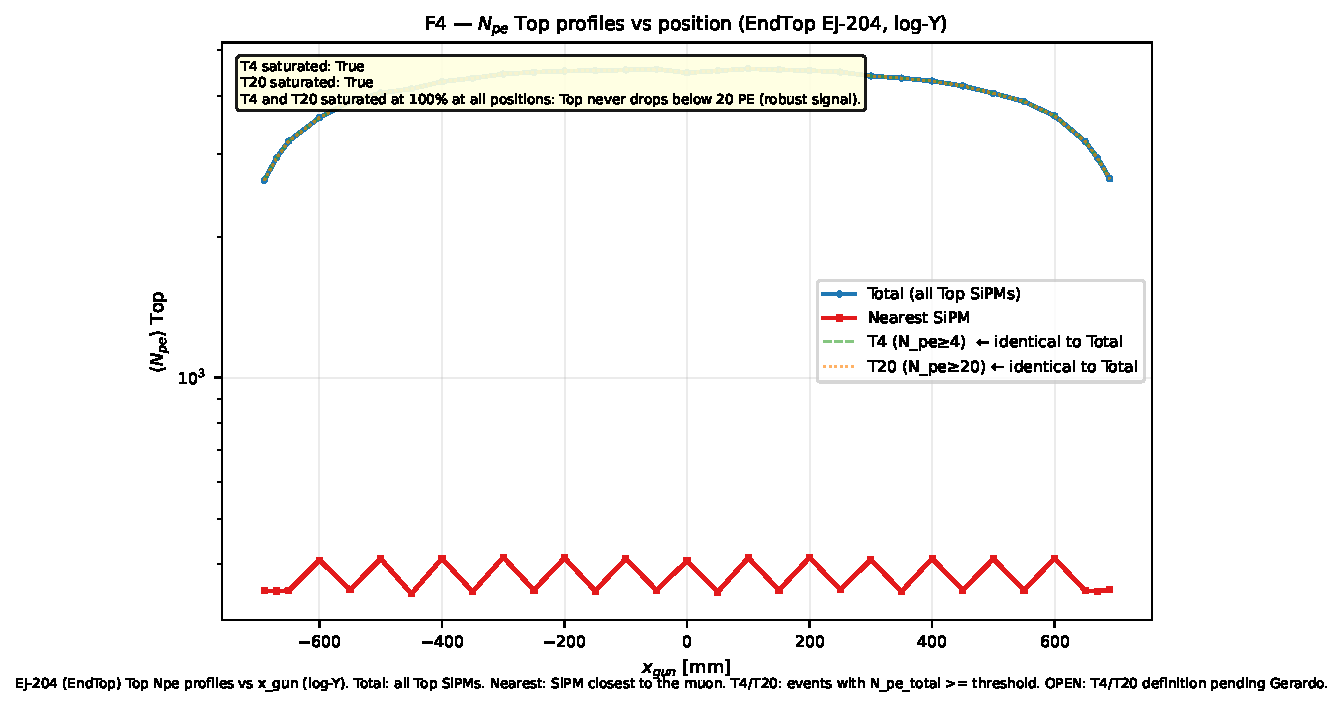
\includegraphics[width=0.74\textwidth,keepaspectratio]{fig04.pdf}

  \begin{itemize}
    \item \textbf{TOP SiPMs} (IDs 16–85): Y-axis = light yield (\emph{not} timing;
          for $\sigma_t$ see F2/F5).
          T4 and T20 \textbf{saturated at 100\%} at all positions: Top never falls
          below 20\,PE — robust signal across the full range.
    \item ``Nearest'' curve oscillates with the discrete \SI{20}{\mm} SiPM pitch.
    \item {\color{pendgold}\textbf{Open — Gerardo:}}
          Is T4/T20 a cut on total $N_\text{pe}$ (as implemented) or a SUM4 trigger efficiency?
  \end{itemize}
\end{frame}

% ══════════════════════════════════════════════════════════════════════════════
\section{Timing resolution SUM4 — F5}

\begin{frame}{F5: SUM4 L/R timing resolution — \textcolor{ej204col}{EJ-204}}
  \framesubtitle{$\sigma_t=\sigma(\Delta T_{LR})/\sqrt{2}$;\quad
    jitter 20\,ps/hit (Stage~1);\quad no time-walk or readout jitter}
  \centering
  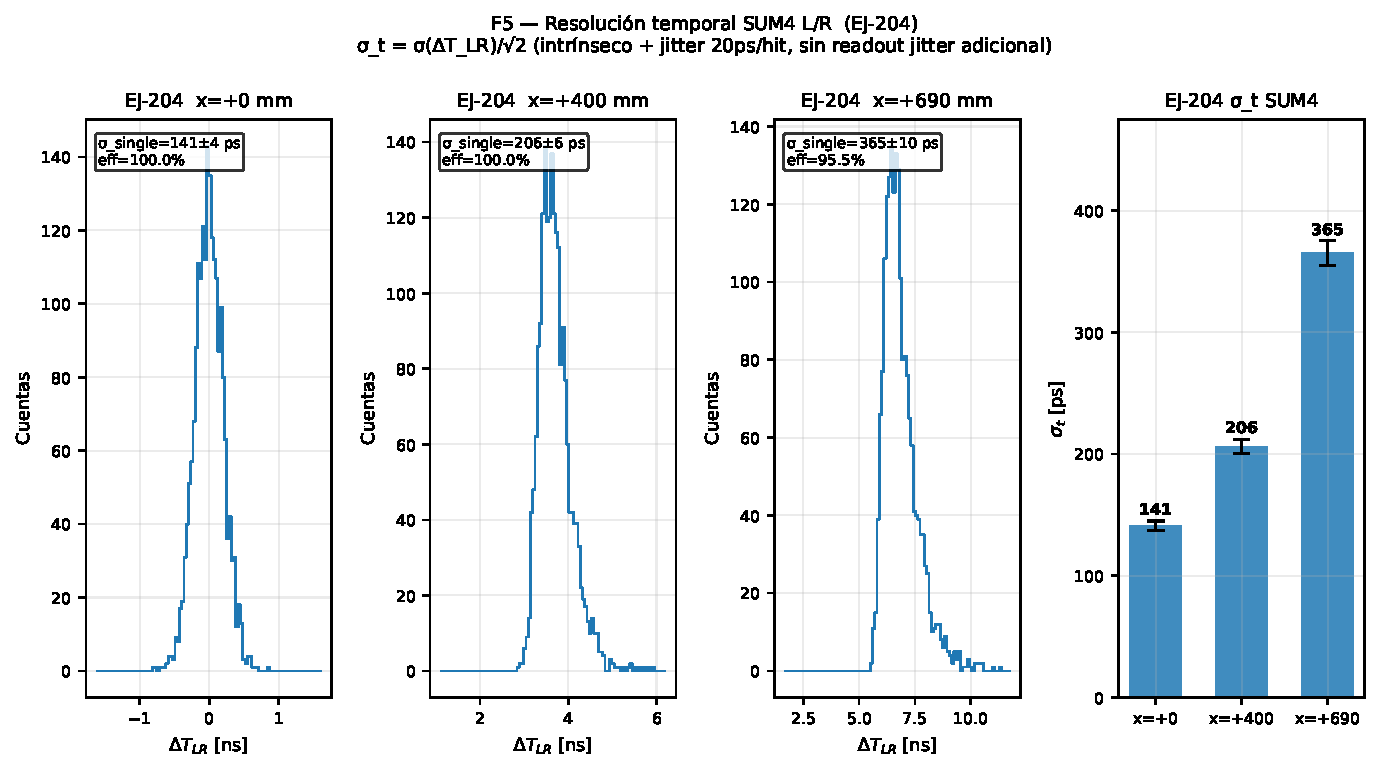
\includegraphics[width=0.76\textwidth,keepaspectratio]{fig05a.pdf}
\end{frame}

\begin{frame}{F5: SUM4 L/R timing resolution — \textcolor{ej230col}{EJ-230}}
  \framesubtitle{$\sigma_t=\sigma(\Delta T_{LR})/\sqrt{2}$;\quad
    same Stage~1 caveats — stronger positional degradation than EJ-204}
  \centering
  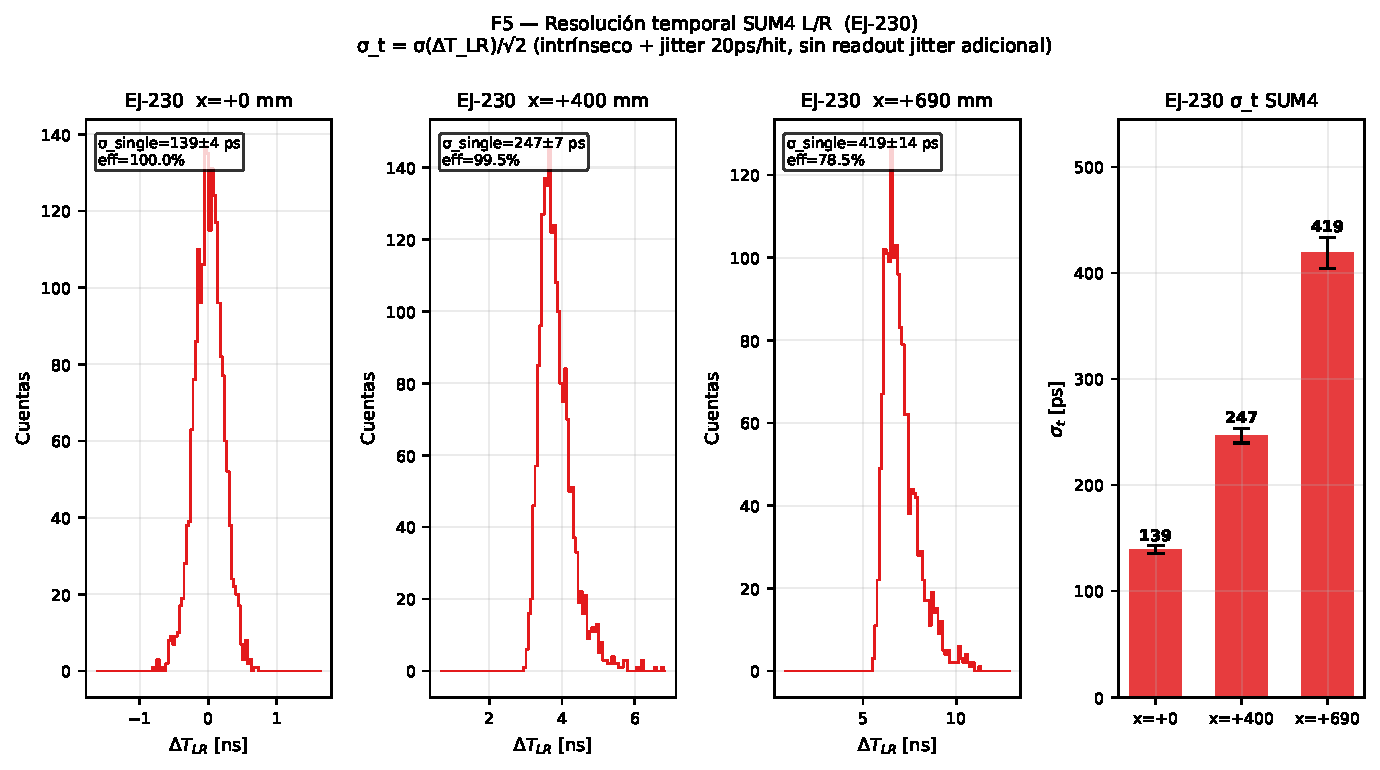
\includegraphics[width=0.76\textwidth,keepaspectratio]{fig05b.pdf}
\end{frame}

\begin{frame}{Timing resolution comparison: EJ-204 vs EJ-230}
  \begin{center}
    \large
    \begin{tabular}{lrrr}
      \toprule
      Material & $x=0$\,mm & $x=+400$\,mm & $x=+690$\,mm \\
               & $\sigma_t$ [ps] & $\sigma_t$ [ps] & $\sigma_t$ [ps] \\
      \midrule
      \textcolor{ej204col}{\textbf{EJ-204}} & $141\pm4$ & $206\pm6$ & $365\pm10$ \\
      \textcolor{ej230col}{\textbf{EJ-230}} & $139\pm4$ & $247\pm7$ & $419\pm14$ \\
      \bottomrule
    \end{tabular}
  \end{center}
  \vspace{0.4em}
  \begin{columns}[T]
    \begin{column}{0.52\textwidth}
      \textbf{Key observations:}
      \begin{itemize}
        \item Central resolution \textbf{equivalent}: $141\approx139$\,ps
        \item EJ-204 $\sim15\%$ better at the edge ($365$ vs $419$\,ps)
        \item EJ-230 degrades faster with position\\
              ($+201\%$ vs $+159\%$ from $x=0$ to $x=690$)
        \item Fitted $\tau_f$: arrival-time profile (emission $\otimes$\ propagation)\\
              \textit{not} datasheet constants\\
              (EJ-204: $\tau_r^{(0)}=0.7$\,ns, $\tau_d^{(0)}=1.8$\,ns)
      \end{itemize}
    \end{column}
    \begin{column}{0.46\textwidth}
      {\small \color{gray}
      \textit{Caveats — Stage 1 (no real electronics):}
      \begin{itemize}
        \item Jitter 20\,ps/hit: possible double-count (L+R)
        \item No time-walk correction (ToT)
        \item No readout jitter applied
        \item SUM4 topology: pending Gerardo
        \item Recovering emission constants\\
              requires deconvolution — Stage 2
      \end{itemize}
      }
    \end{column}
  \end{columns}
\end{frame}

% ══════════════════════════════════════════════════════════════════════════════
\section{Top SiPM redundancy — F6}

\begin{frame}{F6: Top SiPM redundancy — $N_\text{pe}$ correlation between neighbors}
  \centering
  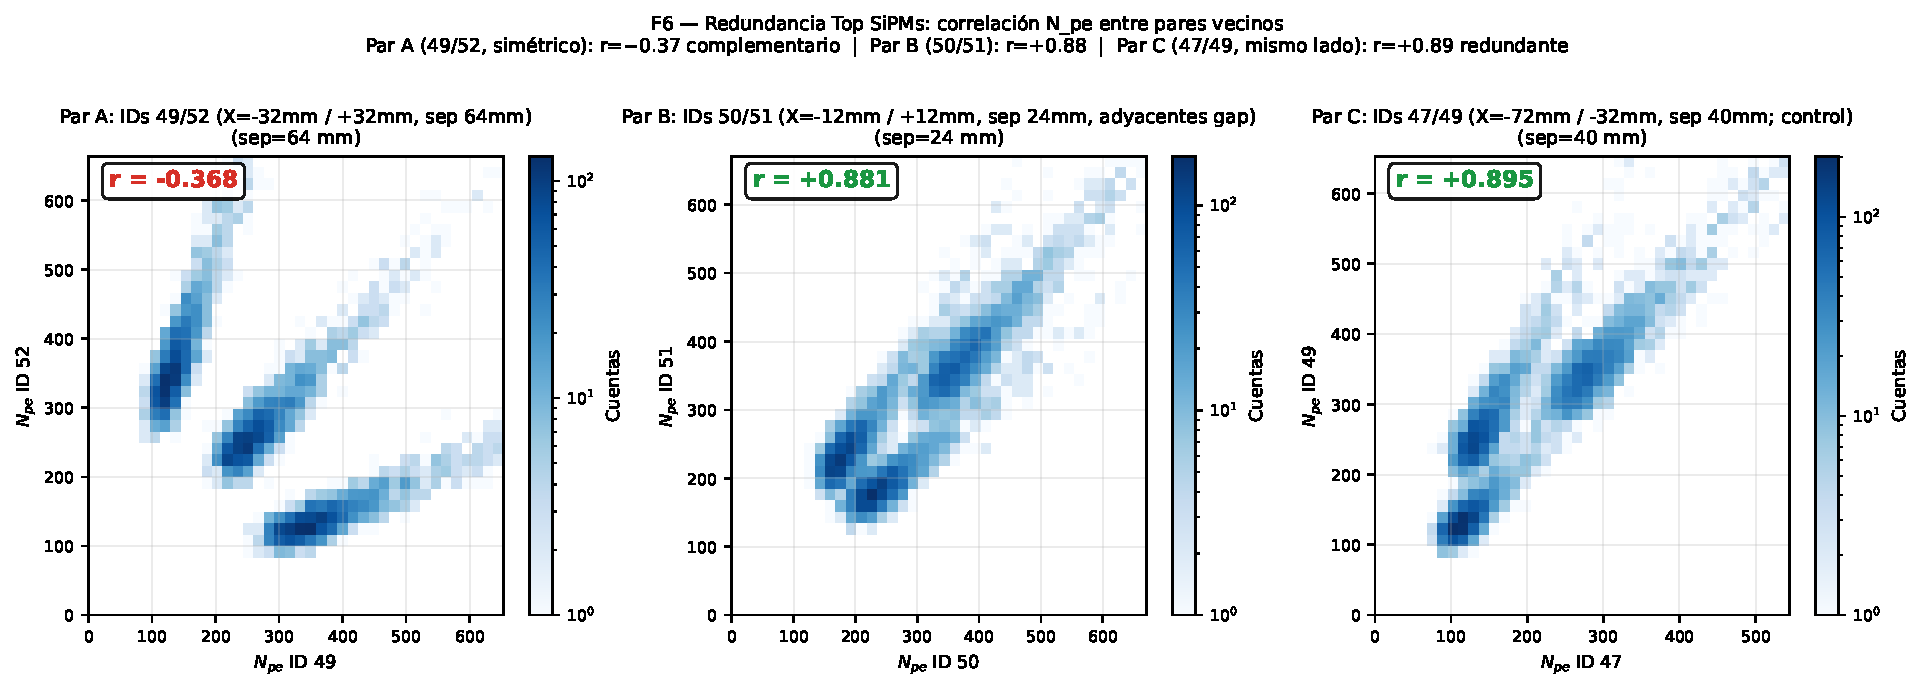
\includegraphics[width=0.88\textwidth,keepaspectratio]{fig06.pdf}

  \smallskip
  \begin{columns}[T]
    \begin{column}{0.32\textwidth}
      \centering
      \textbf{Pair A (IDs 49/52)}\\
      sep $=64$\,mm, opposite sides\\
      $r=-0.37$ — complementary\\
      {\footnotesize (light splits between sides)}
    \end{column}
    \begin{column}{0.32\textwidth}
      \centering
      \textbf{Pair B (IDs 50/51)}\\
      sep $=24$\,mm, across gap\\
      $r=+0.88$ — \textbf{redundant}\\
      {\footnotesize (same light source)}
    \end{column}
    \begin{column}{0.32\textwidth}
      \centering
      \textbf{Pair C (IDs 47/49)}\\
      sep $=40$\,mm, same side\\
      $r=+0.90$ — \textbf{control}\\
      {\footnotesize (local correlation expected)}
    \end{column}
  \end{columns}
\end{frame}

% ══════════════════════════════════════════════════════════════════════════════
\section{Optical path dispersion — F7}

\begin{frame}{F7: Order-statistic arrival time $\langle t_n\rangle$ per Top channel —
              $x=-690$\,mm}
  \framesubtitle{Statistical floor $\sqrt{n}\,\tau_d/\langle N_\text{pe}\rangle$
    ($\tau_d=1.8$\,ns, EJ-204 datasheet); gap = optical path dispersion}
  \begin{columns}[c]
    \begin{column}{0.60\textwidth}
      \centering
      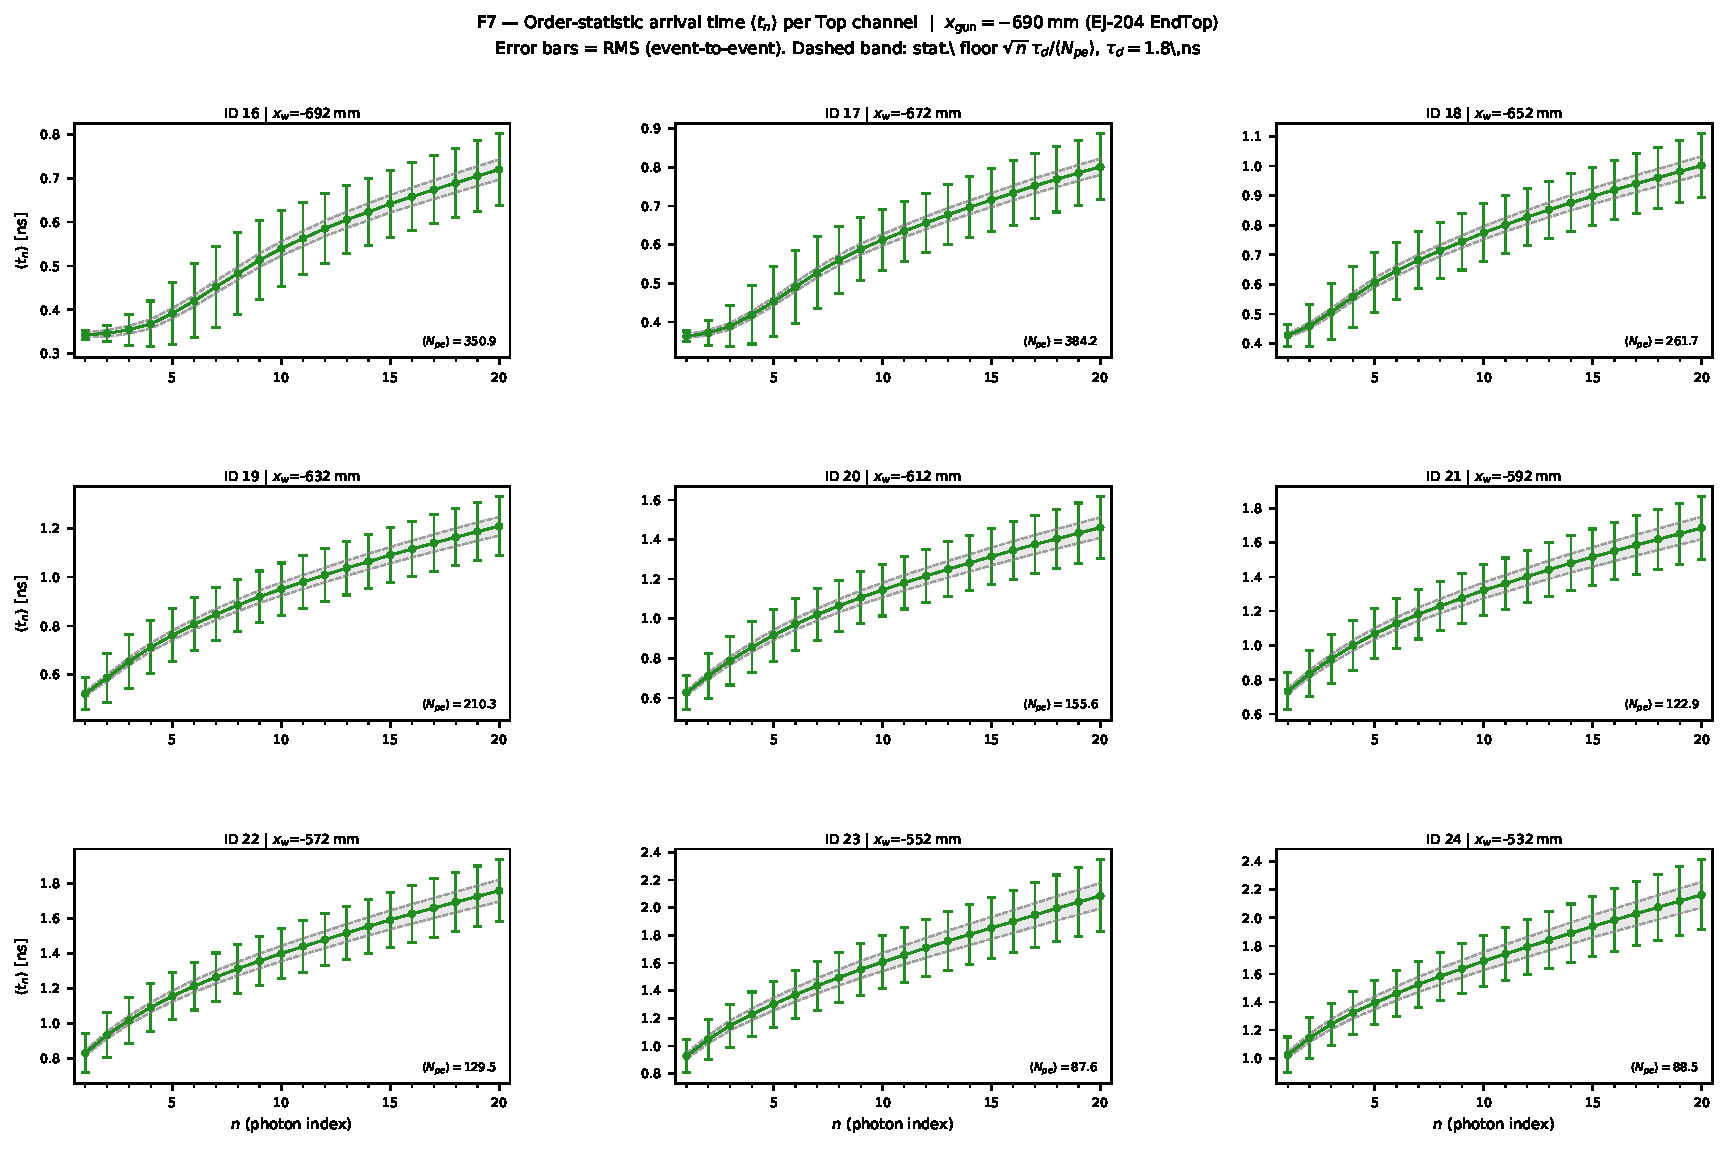
\includegraphics[width=\textwidth,keepaspectratio]{fig07.pdf}
    \end{column}
    \begin{column}{0.38\textwidth}
      \textbf{What the axes show:}
      \begin{itemize}
        \item $x$-axis: $n$ = index of the $n$-th detected photon (order statistic)
        \item $y$-axis: $\langle t_n\rangle$ [ns] — mean arrival time per event
        \item Error bars: RMS over events
        \item Band: statistical floor
              $\sigma_\text{stat}(t_n) = \sqrt{n}\,\tau_d/\langle N_\text{pe}\rangle$
      \end{itemize}
      \vspace{0.3em}
      \textbf{Physics:}\\
      {\footnotesize
        $\text{RMS} - \sigma_\text{floor}$ isolates
        \textbf{optical path dispersion} — the same spread that broadens $\sigma_t$
        and shifts $v_\text{eff}^\text{onset}$ vs nominal.\\[0.2em]
        At $x=-690$: cluster uses IDs 16–24
        ($x_w=-692\to-532$\,mm) — truncated at the left edge; no channels further left.\\[0.3em]
        {\tiny\textit{F7\,\&\,F2 consistent}: dispersion EXISTS here
        (RMS\,>\,floor) but is subdominant to Poisson statistics
        in the SUM4 $\sigma_t$ over the accessible $N_{pe}$ range
        ($b\!\approx\!0$ in F2).}}
    \end{column}
  \end{columns}
\end{frame}

% ══════════════════════════════════════════════════════════════════════════════
\section{Summary}

\begin{frame}{Summary and open questions}
  \begin{columns}[T]
    \begin{column}{0.54\textwidth}
      \textbf{Main results:}
      \begin{enumerate}
        \item \textcolor{ej204col}{\textbf{EJ-204}} $\approx$
              \textcolor{ej230col}{\textbf{EJ-230}} at center ($141$ vs $139$\,ps);
              EJ-204 \textbf{better at edges} ($365$ vs $419$\,ps at $x=690$)

        \item F1 component at $\sim4.7$\,ns at $x=690$ =
              \textcolor{okgreen}{\textbf{geometric ToF}} from far end
              (QA-1c, $\delta=-5\%$). Not slow scintillation.

        \item $v_\text{eff}^\text{nominal}=277$\,mm/ns;
              onset gives $v_\text{eff}^\text{onset}\approx292$\,mm/ns ($+5\%$)
              — fastest optical paths set the onset

        \item F7: $\langle t_n\rangle$ RMS exceeds the statistical floor
              (order-statistics limit) — quantifies optical path dispersion;
              same physics as $\sigma_t$ degradation toward edges

        \item Top: robust $>20$\,PE; gap-adjacent SiPMs
              highly correlated ($r\approx0.88$)
      \end{enumerate}
    \end{column}
    \begin{column}{0.44\textwidth}
      \textbf{\color{pendgold} Open — Gerardo confirmation:}
      \begin{itemize}
        \item[$\square$] SUM4 topology:
              winner-takes-first vs cluster sum
        \item[$\square$] T4/T20: $N_\text{pe}$ cut or trigger efficiency
        \item[$\square$] Jitter 20\,ps: single or double-count (L+R)
        \item[$\square$] F3: SiPM impacts vs volume trajectories
        \item[$\square$] Pair A ($r=-0.37$):
              geometric or reflections
        \item[$\square$] EJ-230 tail at $x=0$:
              slow mode or reflections?
      \end{itemize}
      \vspace{0.3em}
      \textbf{Next steps:}
      \begin{itemize}
        \item EJ-230 EndTop dataset (Top response)
        \item Stage 2: time-walk, readout jitter, real electronics
        \item Deconvolution: emission constants from arrival profiles
      \end{itemize}
    \end{column}
  \end{columns}
\end{frame}

\end{document}
